\documentclass[../PHYS306Notes.tex]{subfiles}

\begin{document}
\section{Lecture 17}
\subsection{Lecture Notes - Rotational Motion of Rigid Bodies}
\subsubsection{Review of Center of Mass - Clickers}
A system of $n$ particles is described by the masses and positions of each particle, $m_\alpha, \v{r}_\alpha$. The total mass is $M = \sum_{\alpha}m_\alpha$. What is the center of mass of the system?
\begin{s}
The center of mass is the weighted positional average of the position vectors (weighted by the masses, normalized by the total mass). It is given by $\v{R} = \frac{1}{M}\sum_{\alpha}m_\alpha\v{r}_{\alpha}$
\end{s}
Consider particles $\alpha$ and $\beta$, and the internal force $\v{F}_{\alpha\beta}$
(the force on particle $\alpha$ due to particle $\beta$). How does Newton's third law relate the internal forces?
\begin{s}
$\v{F}_{\alpha\beta} = -\v{F}_{\beta\alpha}$
\end{s}
\begin{center}
    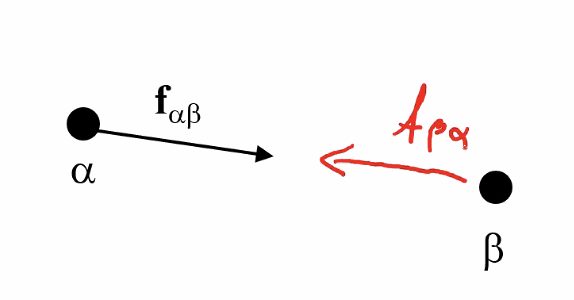
\includegraphics[scale=0.5]{Lecture-17/l17-img1.png}
\end{center}
Suppose a system of particles experiences only internal forces (no external forces). What can we say of the linear momentum of the system?
\begin{s}
The momentum of the COM is constant; the momentum of individual particles can change due to internal forces, but the lack of external forces means the center of mass will have conserved momentum. 
\end{s}

\subsubsection{Linear and Angular Momentum of COM}
We have that the center of the mass position vector is:
\[\v{R} = \frac{1}{M}\sum_{\alpha}m_\alpha\v{r}_\alpha\]
Then the momentum of the center of mass is:
\[\v{P} = M\dot{\v{R}} = \sum_{\alpha}m_\alpha\dot{\v{r}}_{\alpha}\]
The external force is given by:
\[\v{F}_{ext} = M\ddot{\v{R}}\]
We can resolve the motion of the body into the motion of the center of mass and motion relative to the center of mass. Define $\v{r}_\alpha$ (the position vector of one of the point masses that makes up the body) as:
\[\v{r}_\alpha = \v{R} + \v{r}_\alpha'\]
Where the primed coordinates are in the COM frame. The total angular momentum is given by:
\[\v{L} = \sum_\alpha\v{l}_\alpha = \sum_\alpha\v{r}_\alpha \times m_\alpha \dot{\v{r}}_\alpha\]
We substitue $\v{r}_\alpha$ with our expression above, which yields four terms:
\[\v{L} = \sum_\alpha \v{R} \times m_\alpha\v{\dot{R}} + \sum_\alpha \v{R} \times m_\alpha\dot{\v{r}}_\alpha' + \sum_\alpha \v{r}_\alpha' \times m_\alpha \dot{\v{R}} + \sum_\alpha \v{r}_\alpha' + m_\alpha \dot{\v{r}}'\]
What can we say of the quantity $\sum_\alpha m_\alpha\v{r}_\alpha'$?
\begin{s}
Evidently, $\sum_\alpha m_\alpha\v{r}_\alpha' = \v{0}$ as the sum of the relative positions to the COM weighted by the masses would be zero by definition of the COM!
\end{s}
This makes two of our terms in the above sum vanish (namely, the second and third terms). This leaves us with:
\[\v{L} = \sum_\alpha \v{R} \times m_\alpha\v{\dot{R}} + \sum_\alpha \v{r}_\alpha' + m_\alpha \dot{\v{r}}'\]
The first term we may rewrite as $\v{R} \times M\dot{\v{R}} = \v{R} \times \v{P}$, i.e. the angular momentum of the center of mass. The other term is the angular momentum relative to the center of mass. This is a nice decomposition; any angular momentum we can write as:
\[\v{L} = \v{L}_{orbital} + \v{L}_{spin}\]
For example, with the Earth-sun system, we have:
\begin{center}
    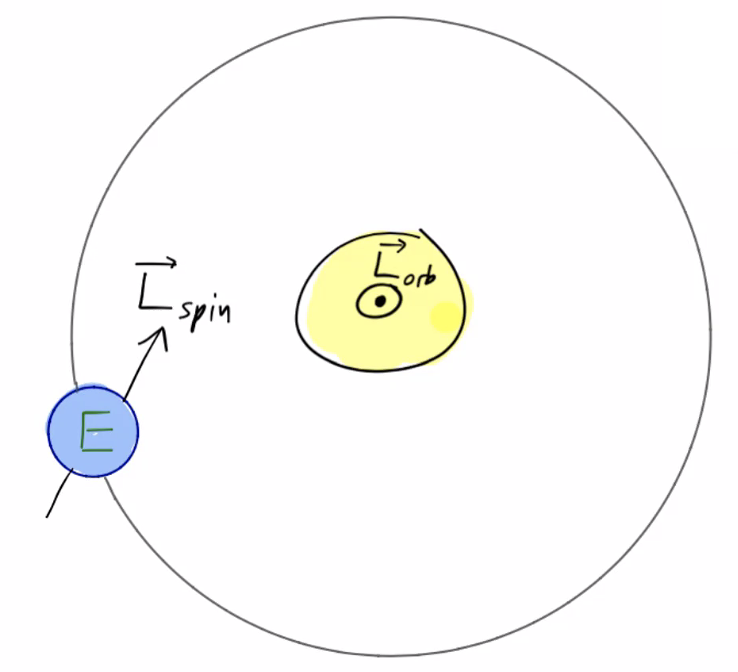
\includegraphics[scale=0.5]{Lecture-17/l17-img2.png}
\end{center}
\subsubsection{Potential and Kinetic Energy of a Rigid Body}
We can also decompose the potential energy of a rigid body:
\[U = U_{ext} + U_{int}\]
Where:
\[U_{int} = \sum_{i < j} U_{ij}(r_{ij})\]
But since in a rigid body all particle distances $r_{ij}$ are fixed, the internal potential energy $U_{int}$ must be constant!
\newline Consider particles $\alpha$ and $\beta ;$ the internal force $\mathbf{f}_{\alpha \beta}=$ the force on particle $\alpha$ due to particle $\beta ;$ the position vector $\mathbf{r}_{\alpha \beta}=$ the vector from particle $\alpha$ to particle $\beta .$ If the force between the two particles is central, what can you say about $\mathbf{r}_{\alpha \beta} \times \mathbf{f}_{\alpha \beta} ?$
\begin{center}
    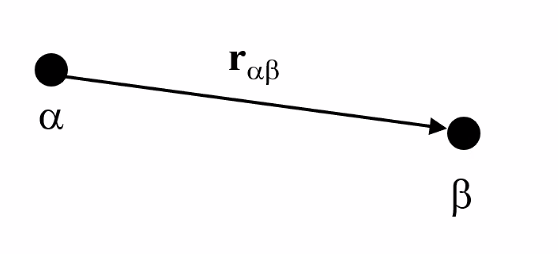
\includegraphics[scale=0.5]{Lecture-17/l17-img3.png}
\end{center}
\begin{s}
Since the vectors would be parallel in the case of central forces, $\v{r}_{\beta\alpha} \times \v{f}_{\alpha\beta} = \v{0}$, that is internal central forces do not change the angular momentum.
\end{s}
A system of n particles is described by the masses and positions of each particle, relative to the center of mass: $\mathrm{m}_{\alpha}, \mathbf{r}_{\alpha}^{\prime}$ The squared velocity of each particle is therefore
$$
\mathrm{v}_{\alpha}^{2}=\dot{\mathbf{r}}_{\alpha}^{\prime 2}+2 \dot{\mathbf{r}}_{\alpha}^{\prime} \cdot \dot{\mathbf{R}}+\dot{\mathbf{R}}^{2}=\mathrm{v}_{\alpha}^{\prime 2}+2 \dot{\mathbf{r}}_{\alpha}^{\prime} \cdot \dot{\mathbf{R}}+\mathrm{V}^{2}
$$
What is the total kinetic energy of the system?
\begin{s}
$\mathrm{T}=\frac{1}{2} \sum_{\alpha} \mathrm{m}_{\alpha} \mathrm{v}_{\alpha}^{\prime 2}+ \sum_\alpha m_\alpha \v{v}_\alpha' \cdot \v{V} + \frac{1}{2} \mathrm{MV}^{2} $ But the second term vanishes by the same previous argument, so:
$\mathrm{T}=\frac{1}{2} \sum_{\alpha} \mathrm{m}_{\alpha} \mathrm{v}_{\alpha}^{\prime 2}+\frac{1}{2} \mathrm{MV}^{2}$ Where we can see that the kinetic energy can also be decomposed to the kinetic energy of the center of mass, and the kinetic energy relative to the center of mass. 
\end{s}
Note that for the kinetic energy about an instantaneous axis of rotation of a rigid body, we have
\[T = \frac{1}{2}\sum_\alpha m_\alpha \dot{\v{r}}^{'2}_\alpha\]
Where we have chosen the center of mass $\v{R}$ to be a point of the body at rest (and hence $\dot{\v{R}} = 0$). 
\subsubsection{Example: Rolling Disk}
\begin{center}
    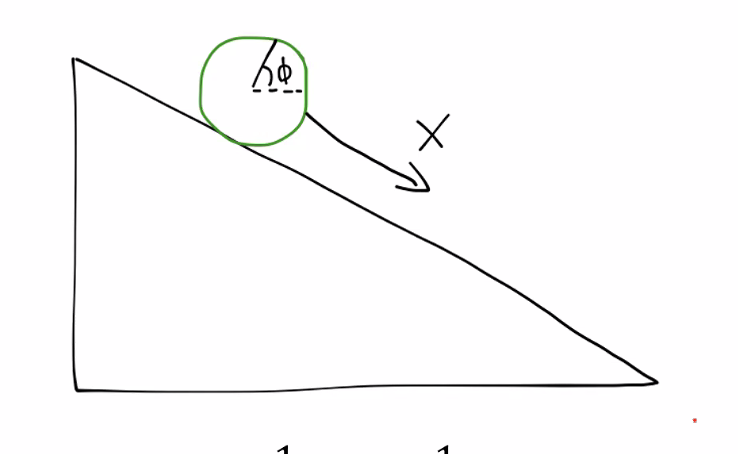
\includegraphics[scale=0.5]{Lecture-17/l17-img4.png}
\end{center}
The kinetic energy of a disk rolling down an incline is given by:
\[T = \frac{1}{2}m\dot{x}^2 + \frac{1}{2}I\dot{\phi}^2\]
Where $I$ is the moment of inertia about the central axis.

\subsubsection{Rotation about the z axis}
\begin{center}
    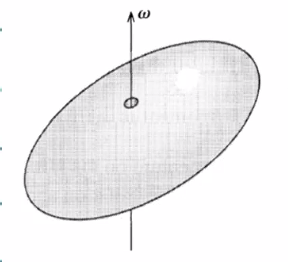
\includegraphics[scale=1]{Lecture-17/l17-img5.png}
\end{center}
In this case, the angular momentum and kinetic energy are given by:
\[\v{L} = \sum_\alpha \v{r}_\alpha \times m_\alpha \v{v}_\alpha\]
Where:
\[\v{v}_\alpha = \v{\omega} \times \v{r}_\alpha = \m{0 \\ 0 \\ \omega} \times \m{x_\alpha \\ y_\alpha \\ z_\alpha} = \m{-\omega y_\alpha \\ \omega x_\alpha \\ 0}\]
Hence:
\[m_\alpha \v{r}_\alpha \times \v{v}_\alpha = m_\alpha \m{x_\alpha \\ y_\alpha \\ z_\alpha} \times \m{-\omega y_\alpha \\ \omega x_\alpha \\ 0} = m_\alpha\omega\m{-z_\alpha x_\alpha \\ -z_\alpha y_\alpha \\ x_\alpha^2 + y_\alpha^2}\] 
$x_\alpha^2 + y_\alpha^2$ is just the distance from the rotation axis, so identify it as $\rho_\alpha^2$. Then, the z component of the angular momentum is given by:
\[L_{z} = \sum_\alpha m_\alpha\rho_\alpha^2\omega = I_{zz}\omega\]
The double $zz$ notation will become clear in a moment. \newline Next, let's look at the kinetic energy $T = \frac{1}{2}\sum_\alpha m_\alpha v_\alpha^2$. Since we are doing circular motion about a rotational axis, $v_\alpha = \omega \rho_\alpha$. Hence:
\[T = \frac{1}{2} \sum_\alpha m_\alpha\omega^2 \rho_\alpha^2 = \frac{1}{2}I_{zz}\omega^2\]
Next looking at the other components of the angular momentum, we have
\[L_x = -\sum_\alpha m_\alpha x_\alpha z_\alpha \omega, \quad L_y = -\sum_\alpha m_\alpha y_\alpha z_\alpha \omega\]
We now define some new quantities:
\[L_x = -I_{xz}\omega, \quad L_y = -I_{yz}\omega\]
We see that $\omega$ only has one component (in the z direction), but evidently, the angular momentum has more than one component, and hence is not parallel to omega! In the past (e.g. first year physics) we have only studied problems where $\v{L}$ is parallel to $\v{\omega}$ but here this is definitely not the case.
\newline We note that $I_{ij}$ are the products of inertia. This can be generalized to three dimensions, by introducing the inertia matrix/tensor:
\[\v{L} = \II\bm{\omega}\]
It is no longer sufficient to treat the moment of inertia as a single number.
\newline What is the direction of $\v{L}$ of $m$ at this moment pictured?
\begin{center}
    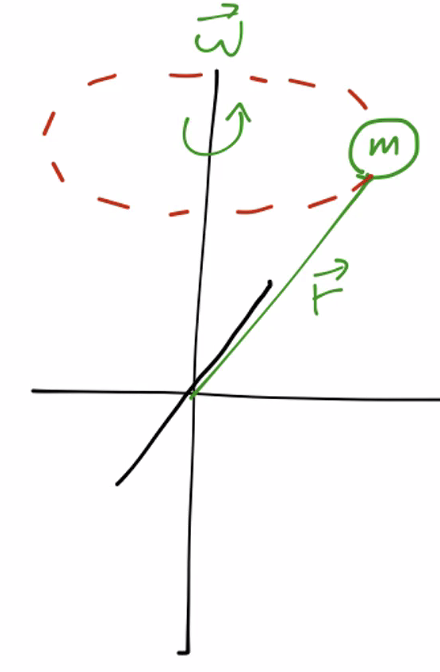
\includegraphics[scale=0.5]{Lecture-17/l17-img6.png}
\end{center}
\begin{s}
The velocity is into the page, and the position vector points up and right, so evaluating $\v{l} = \v{r}\times\v{v}$ (with the RHR), we get that the direction is up and left.
\end{s}
Now considering the same setup as above, what happens to $\v{L}$ and the moment of inertia $\II$ as the mass spins around?
\begin{s}
As the mass rotates around the axis, the direction of the angular momentum will change. Since $\bm{\omega}$ is constant in time, we must have that $\II$ changes in time by $\v{L} = \II\bm{\omega}$. Hence, $\v{L}$ and $\II$ both change, and there is a net torque on the mass. There will only be some special axis for which the moment of inertial will not change (e.g. the wheel rolling down the inclined plane). But in general, $\v{L}$, $\II$ are not invariant in time. 
\end{s}
\begin{center}
    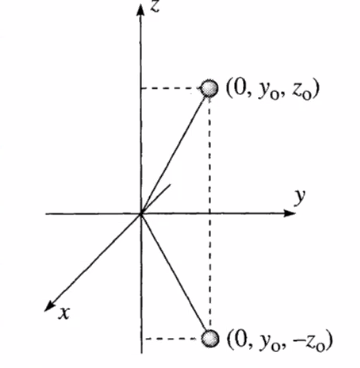
\includegraphics[scale=0.5]{Lecture-17/l17-img7.png}
\end{center}
For the shown configuration, what are the products of inertia for rotation about the z axis? Using the formulas we derived previously, we have:
\[I_{zz} = \sum_\alpha m_\alpha(x_\alpha^2 + y_\alpha^2) = m(0 + y_0^2 + 0 + y_0^2) = 2my_0^2\]
\[I_{xz} = -\sum_\alpha m_\alpha x_\alpha z_\alpha = 0\]
\[I_{yz} = -\sum_{\alpha}m_\alpha y_\alpha z_\alpha = -m(y_0z_0 + y_0(-z_0)) = 0\]
So in this case, we have that $\bm{\omega} \parallel \v{L}$. Next day, we will look at the general inertia tensor, and perhaps the principle axes of rotation (for which the inertia tensor is simple/diagonal).
\end{document}